\documentclass[a4paper,12pt]{article}
\usepackage{amsmath, amssymb, graphicx}
\graphicspath{ {D:/Library/Meteorology/Note_tex/Symmetric_Instability} }

\DeclareMathAlphabet{\mathcal}{OMS}{cmsy}{m}{n}
\SetMathAlphabet{\mathcal}{bold}{OMS}{cmsy}{b}{n}
\newcommand{\bigO}{\mathcal{O}}


\begin{document}

\title{\vspace{-4.0cm} Static, Inertial and Symmetric Instability}
\author{Ian Beckley
\\University of Wisconsin-Madison}

\date{8 Jan. 2021}

\maketitle

\subsection*{Static Stability}

An environment is characterized as statically stable when $\frac{d\theta}{dz} > 0$ (or, for moist environments, $\frac{d\theta_e}{dz} > 0$). This requires that a vertical parcel displacement is met with a vertical restorative force that opposes displacement. Viewed through the consideration of elementary density, in a statically stable environment a parcel displaced upward (downward) will be cooler (warmer) than its environment and subsequently sink (rise) toward equillibrium. A statically unstable environment is inherently out of hydrostatic balance ($\frac{dp}{dz} \neq -\rho g$) due to non-zero vertical accelerations. Furthermore, statically unstable environments ($\frac{d\theta}{dz} < 0$) are seldom observed. We do observe, however, vertical accelerations due to \emph{conditional} instability. In the case of conditional instability, the environmental lapse rate, $\gamma$, is $\Gamma_m < \gamma < \Gamma_d$ suggesting that a saturated parcel  \emph{can} become unstable relative to the dry adiabatice lapse rate. Put differently, conditional instability is observed when $\frac{d\overline{\theta_e^*}}{dz} < 0$, where $\overline{\theta_e^*}$ is the equivalent potential temperature the environment would have if it was saturated at that temperture and pressure.

\subsection*{Inertial Instability}
While the aformentioned form of parcel instability pertains to the vertical displacements and accelerations, inertial instability leads to horizontal accelerations due to horizontal parcel perturbations. It should be obvious, then, that the equillibrium at hand is that of geostrophic balance ($\frac{du}{dt} = 0$). Geostrophic balance exists between the horizontal pressure gradient force and the coreolis force, both of which can have non-zero spatial derivatives. If a parcel or along-flow tube of parcels is in geostrophic balance in one location, will it still be in geostrophic balance when displaced horizontally to another location? If not, there is a net acceleration vector due to the violation of geostrophic balance which must be investigated. 

Imagine a scenario wherein $\frac{d\,\nabla P}{dy} > 0$, or that the pressure gradient force (and thus $V_g$) increases to the north and the flow is westerly. A parcel displaced to the north will accelerate initially to the right of the displacement due to the increasing coreolis force. At the northward location, however, the PGF is significantly greater than it was initially, thus the parcel is not in geostrophic balance. Since the PGF is greater than the Coreolis force, a horizontal acceleration now forms in the direction of the initial displacement. This represents an inertially unstable scenario. Now suppose that a parcel displaced northward encounters a weakened pressure gradient force at its new location. The parcel will initially torque to the right of displacement due to the coreolis force, however, at the new location the PGF is lesser than the coreolis force such that a restorative acceleration occurs against the direction of dipslacement. This represents an inertially stable situation.

In an analog to potential temperature, inertial instability can be understood by defining a new variable, \emph{absolute momentum}, which is the zonal momentum a parcel would have if moved to the equator, $M = u - fy$. This value is conserved following the motion for a purely zonal geostrophic flow on an $f$ plane, and we can take its gradient in order to asses the instability. Define the geostrophic absolute momentum, $M_g = u_g - fy$. Taking its derivative with respect to y,

\begin{align*}
\frac{\partial M_g}{\partial y} = \frac{\partial u_g}{\partial y} - f
\end{align*}

Inertial instability is present if $\frac{\partial M_g}{\partial y} > 0$. A parcel displaced to the north will have an $M$ value lesser than the local $M_g$ value indicating an imbalance between the PGF and coreolis forces. Under the provided conditions, the coreolis force will be weak relative to the PGF, and the parcel will accelerate in the direction of its displacement. Recall that in the northern hemisphere $f > 0$, and $\frac{\partial u_g}{\partial y} > 0$ corresponds to negative relative vorticity. It follows that inertial instability is present when geostrophic absolute vorticity is negative. This seldom occurs on the synoptic scale, but can frequently occur within inflow regions of convective complexes.

\subsection*{Symmetric Instability}
Parcels can be both inertially and statically stable though unstable to slanted displacements (with respect to the horizontal). See the depiction below (Markowski and Richardson 2010, fig 3.9).

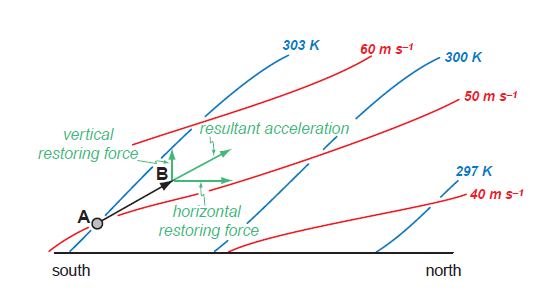
\includegraphics[width=\textwidth]{sym_ins}

 Note that the atmosphere is statically stable (in hydrostatic balance), and inertially stable (lines of constant $M_g$ decrease northward). Take a purely vertical parcel displacement from A. The parcel will subsequently be colder than its surrounding environment and sink bank to its isentrope. Take a purely horizontal displacement from A. The parcel will immedietly encounter lower momentum air, and an imbalanced coreolis force will return the parcel back to geostrophic equillibrium. Each of these restorative scenarios exist for parcel placements steeper than isentropes and slighter than lines of constant momentum. 

Now take a parcel displacement from A to B whose displacement path is between isentropes and lines of absolute momentum. It is easy to see from our prior discussions that a parcel at B is warmer than its environment and has lower momentum than the geostrophic conditions warrant. The parcel will feel a vertical restorative force to re-establish hydrostatic balance, and, likewise, a horizontal restorative force to re-establish geostrophic balance. These restorative forces, however, act simultaneously and subsequently promote an acceleration in the slant-wise direction. This constitutes symmetric instability, which is of great interest since vertical accelerations could warrant precipitation, or even the release of convective potential energy.

Typically moist isentropes exhibit a steeper slope than their dry counterparts due to a lack of moisture aloft. It should be clear that symmetric instability can only be realized when isentropes are steeper than lines of constant absolute momentum, thus one can imagine a scenario wherein an environment is symmetrically stable with respect to dry displacements, but symmetrically unstable with respect to moist displacements. As you may expect, this is known as \emph{conditional} symmetric instability.



\end{document}
